% Robot
\begin{frame}{Robot and controller}
\begin{columns}
\column{.5\textwidth}

\begin{itemize}
\item Controller, (DX100)
\begin{itemize}
\item Controlls the robot (SIA20D)
\item Robot orientation 
\end{itemize}
\end{itemize}

  \column{.5\textwidth}
    \begin{figure}[H]
	\begin{center}
	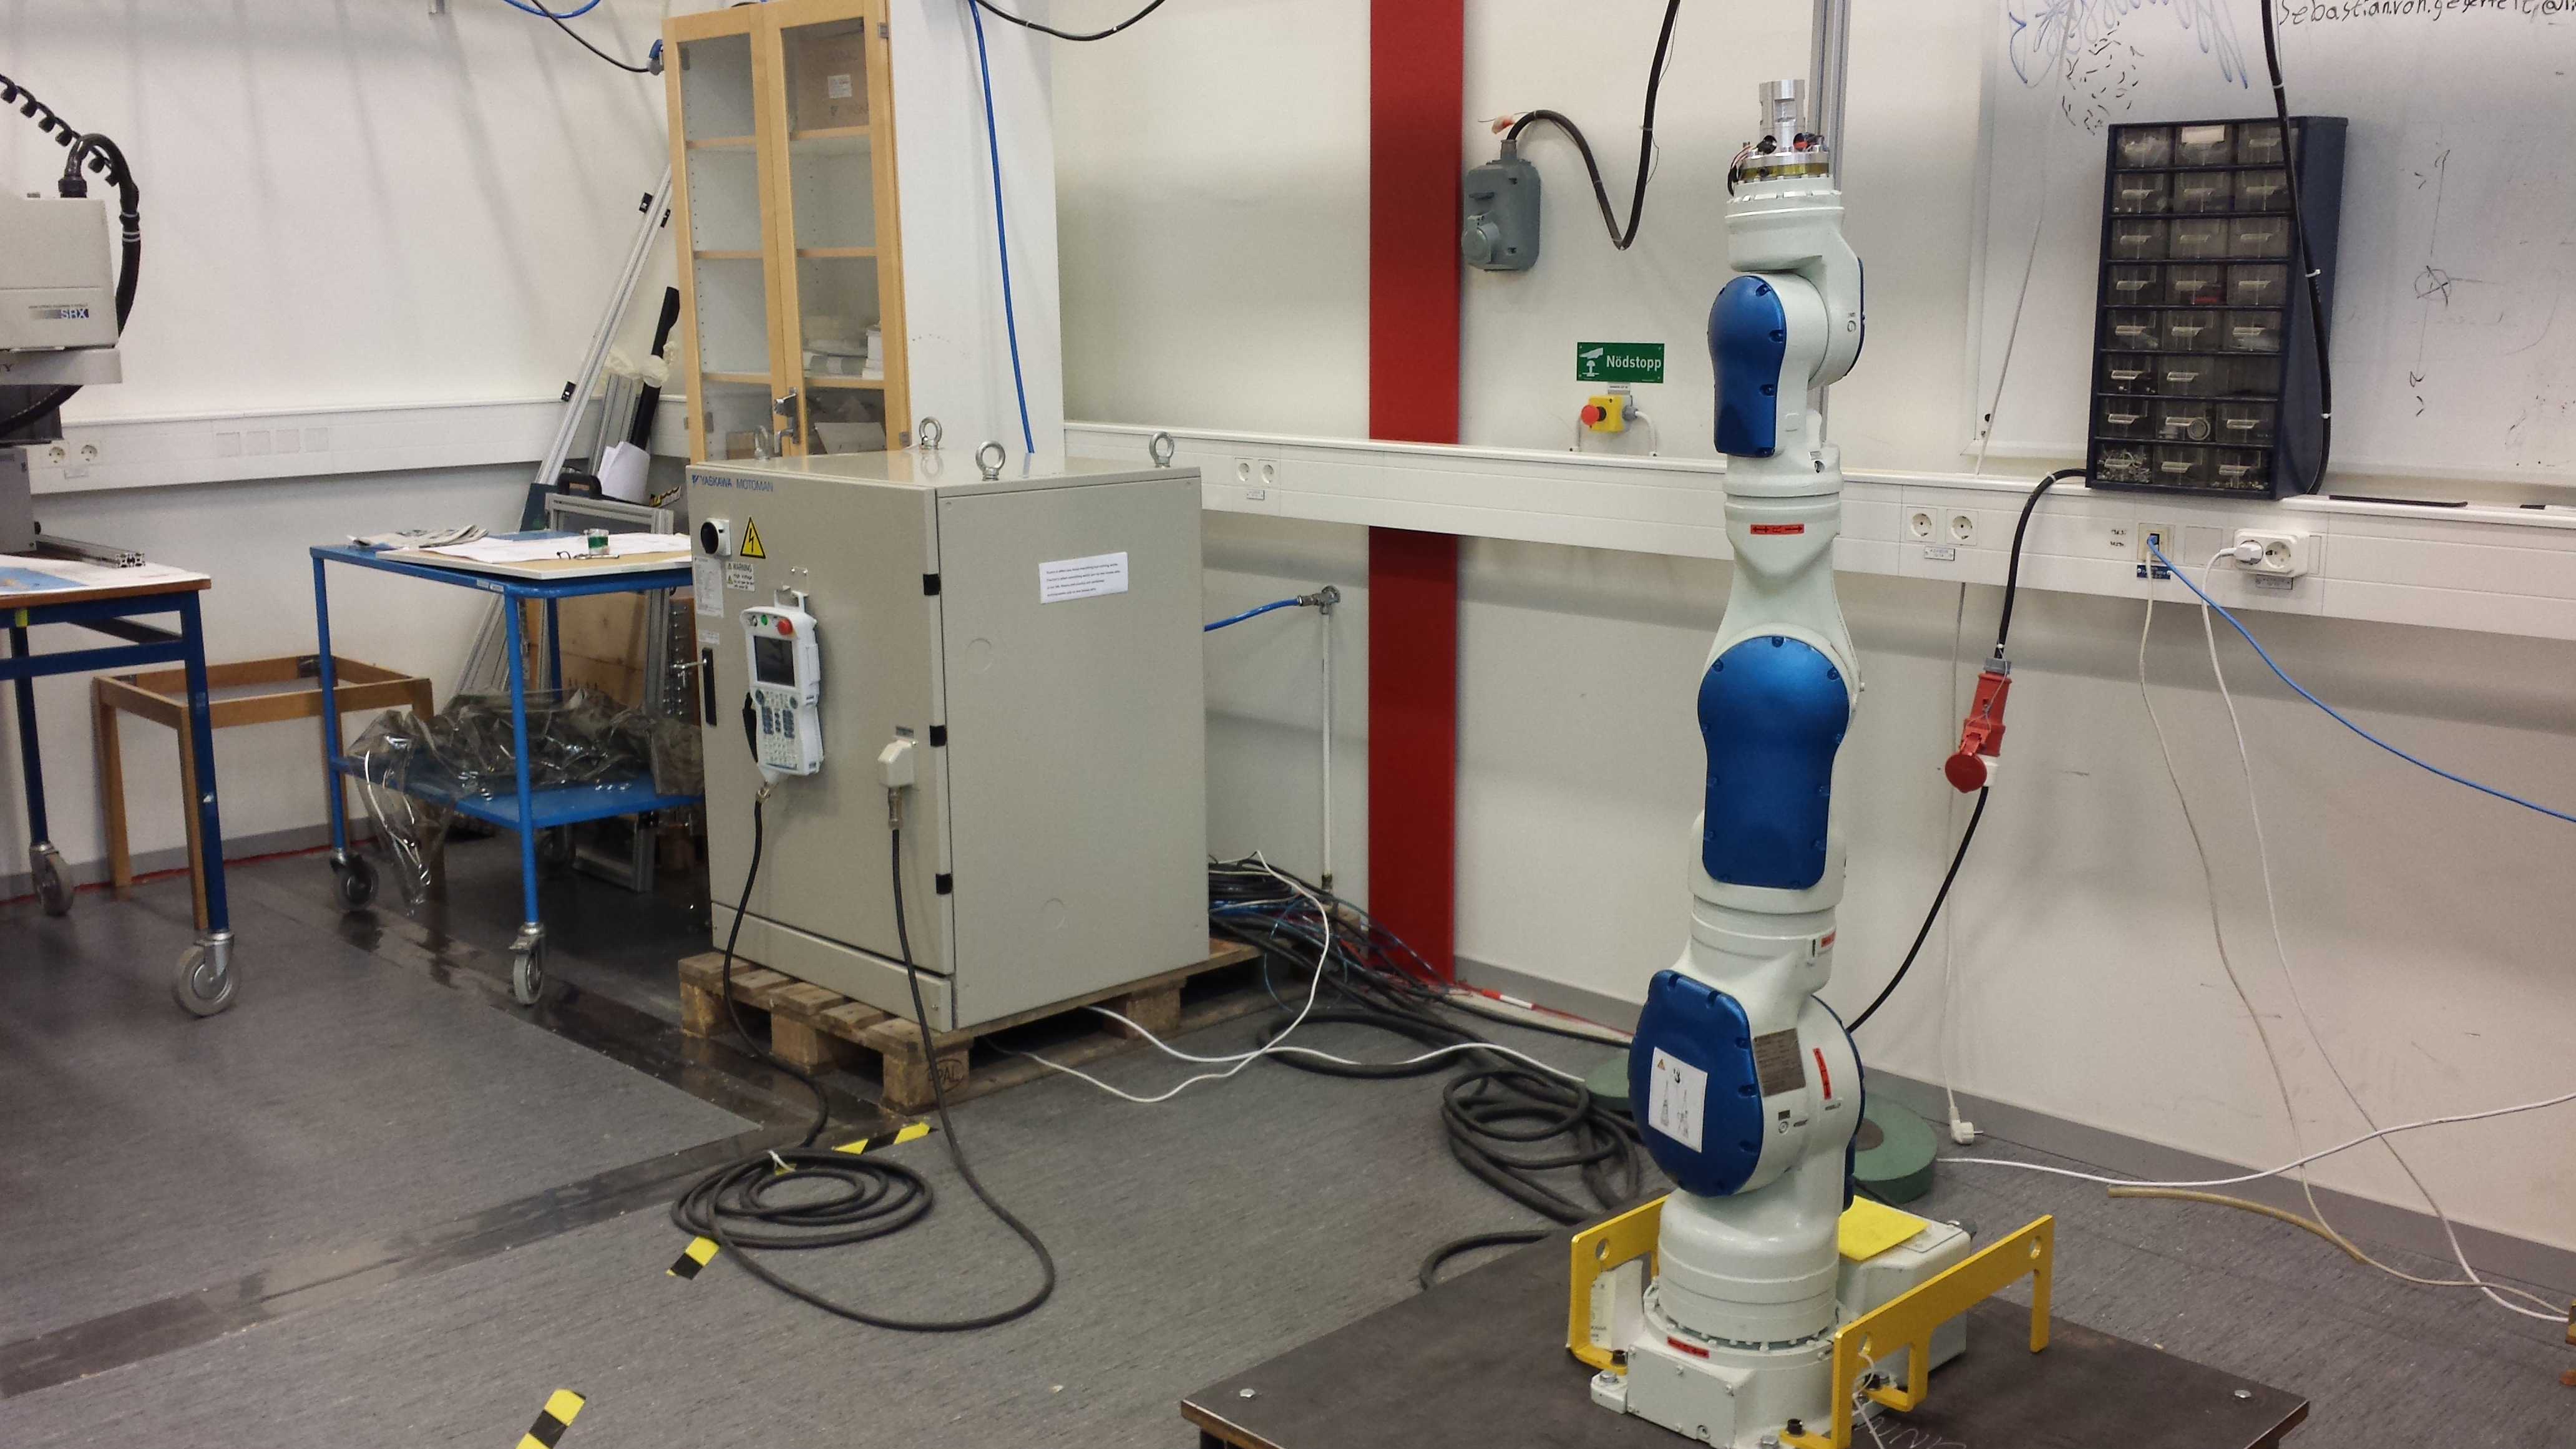
\includegraphics[width=5 cm]{controller}
	\end{center}
	\end{figure}
    \end{columns}

\end{frame}

\begin{frame}{Controller - Computer interface}


\begin{itemize}
\item ROS (Robot Operating System)
\begin{itemize}
	\item Communicate with controller
	\item OpenCV
	\item PCL (point cloud library)
\end{itemize}
\item Joint coordinates to computer
\item ''Send'' motion commands to controller
\end{itemize}

\end{frame}


